\newpage
\section{Methodology}

% Methodology, introduction based on CRISP methodology
The methodology used in this thesis is based on the CRISP-DM methodology, as well as the well known hyper-parameter search performed by cross-validation. Any other insights that are extracted from the data follow the standards of design of experiments and statistical hypothesis modeling.

\begin{figure}[H]
    \centering
        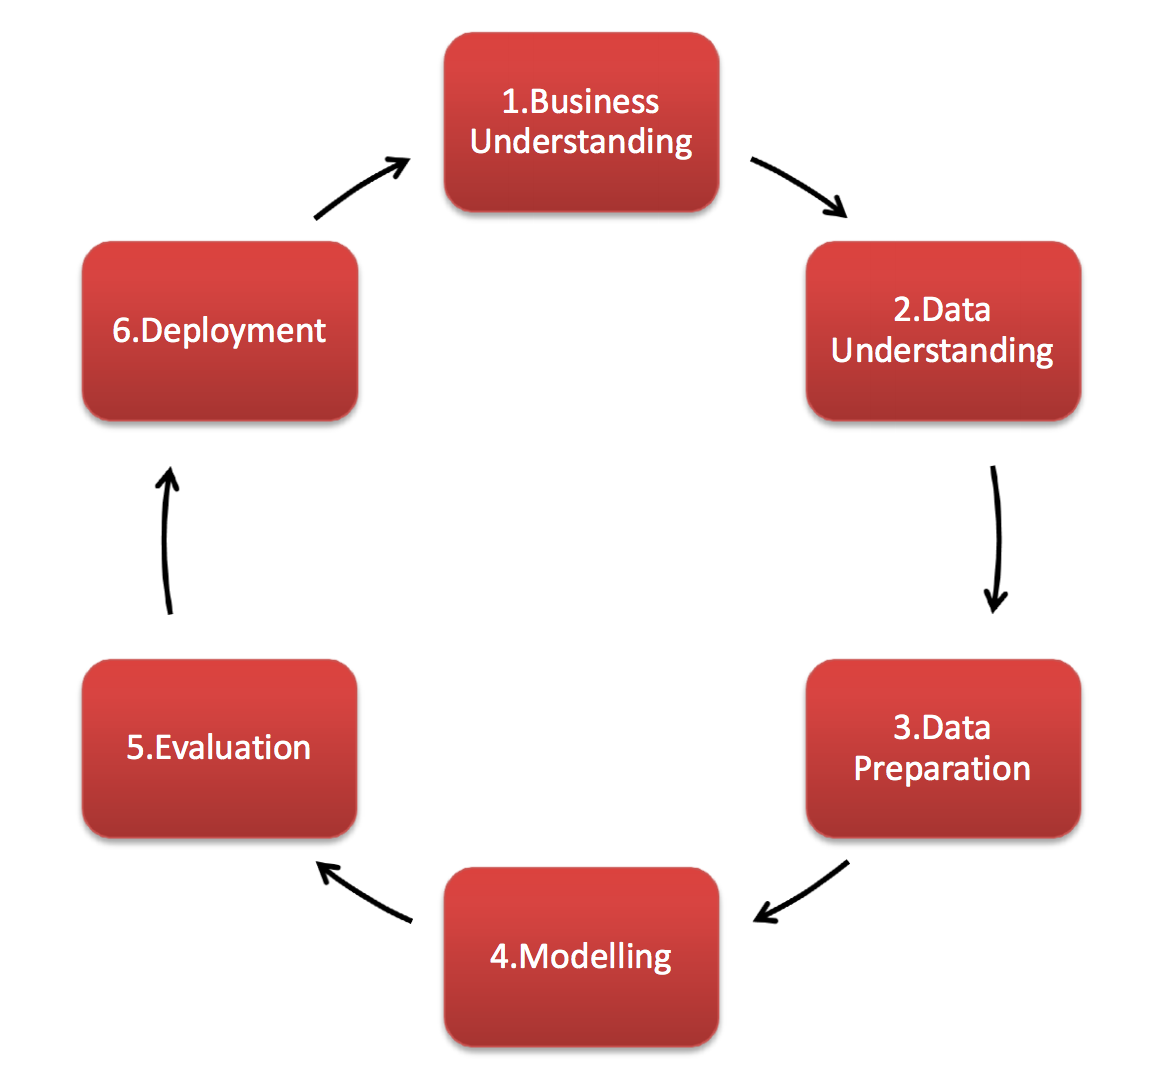
\includegraphics[width=0.6\linewidth]{img/crisp-dm.png}
    \caption{CRISP-DM methodology steps}\label{fig:crisp}
\end{figure}


CRISP-DM is the most representative method to plan the overall data extraction or generation, design of experiments and evaluation. It consists of six major tasks: business understanding, data understanding, data preparation, modeling, evaluation and deployment. Since this thesis has exploratory and research goals, the first and last steps of the CRISP-DM, business understanding and deployment, are not implemented, simple indications are given about them. The following points give an overview of how the CRISP-DM has been implemented in each of the two experiments.

\textbf{Problem understanding}

This steps allows for careful review of the goals and motivations of the thesis and its experiments. It's the place where the experiments to be performed are designed and the desired goals are stated. It gives an indication on how to perform the experiments, with which data, and when to stop.

\textbf{Data understanding}

In this step, the selected data is analyzed to decide which preprocessing actions will be needed, which machine learning tasks are more suitable for it and which results can we expect from it. 
Some insights of the data are performed as a data exploratory analysis. Distributions of features, correlation analysis, generation of aggregations and other basic statistical analysis are performed when necessary.
Specially for the second task of this project for which data is not labeled, data labeling procedures are analyzed and tested at this stage.

\textbf{Data preparation}

In this step, all the needed preprocessing is performed. It consists of the extraction of the actual data, and the execution of data cleaning, where outliers, errors and missing data are corrected in the most suitable way for the problem that needs to be solved. Then the feature selection is performed, where data features are chosen based on the goals and previous analysis. Feature engineering is also performed to come up with transformations of the data that are suitable for the problem at hand.


\textbf{Modelling}

At this stage, data is prepared to be fed to a model training procedure. The model training procedure will consist on performing a search for the best hyper-parameters for each type of model that is intended to be trained. Out of this hyper-parameter search, the best model of each type for the current dataset will be produced as an output. 
The hyper-parameter search is executed by a well-known procedure called cross-validation, where the dataset is split into training, validation and testing. The model is trained on the training split and tested on the validation split until the best set of parameters is found. Then finally, to assess the generalization power of the best model, it is tested again with the test data split. 
The more advanced way to perform the validation is to split only training and testing, and divide the training split into k folds, where k-1 folds are used for training and the remaining fold is used for validation. The average metric score on all the training-validation fold permutations is used to select the best set of parameters.
The two tasks undertaken in this thesis belong to node regression and graph classification. For the node regression, since we want to approximate a real value for nodes of a graph, the normalized root mean squared error is the correct performance metric to use.  However, the problem will be transformed into a classification task by defining ranges of values, thus the correct performance metric will be the accuracy or the f1-score averaged over all classes. For the graph classification task, code subroutines classification, there are many classes with imbalance and so a macro average of precision and recall, namely f1-score, is the right performance metric to use.

\textbf{Evaluation}

In this step the best model of each kind is selected. Part of this tasks, when using cross-validation is already done in the modeling part. But it's in this step when results are presented and compared altogether. 
It is important to stress out that the best model must be chosen by the validation performance metric. The test on the test data split must be used to verify that the model is not over-fitting the validation set, which would indicate that the model will no be able to generalize to unseen data. When the validation performance metric is similar to the test performance metric it indicates that the model should be able to generalize to unseen data.

% \subsection{Deployment}

% This step will only serve as a wrap up of the experiments, concluding on the power of the models tested to model the problem at hand. It will also serve as a place to indicate the next steps in order to improve the modelling, explore new versions of the problem or implement a product that exploits the trained model.
% Baseline models
% 	- simpler models

% Cross-validation training
% 	- cv, folds then retraining
% 	- class-imbalance handled with
% 		- balanced training dataset splits
% 		- useing f1-macro as we want to optimize for overall prec-rec on all classes

% Model selection
% 	using the cv-score (f1-macro)
% 	then showing the generalization capability of the model on the test set (understand if cv score increases also makes the test score do it)